\chapter{\term{HIP} 效能優化} \label{chap:hip_optimization}
在本章中,我們將探討幾種可以提升 GPU 程式效能的策略。我們將以一些具體的 GPU 應用(例如影像伽瑪校正、矩陣乘法)作為範例,並提供實作的方式。接著,我們會比較這些實作的效能,展示各種效能優化方法可能帶來的改善。

在詳細說明具體方法之前,必須先討論 GPU 效能的 portability。一般而言,GPU 的效能的 portability 較為有限。這意味著在一個 GPU 上表現良好的方法,可能因為架構的差異,在另一個 GPU 上未必有相同的效果。因此,程式設計者不應僅依賴單一方法,而是應針對目標 GPU 進行實驗和效能分析,以選擇最有效的優化策略。

\section{高度平行化工作負載 – 影像伽瑪校正}
\label{sec:gamma_correction}
GPU 通常擁有數千個能夠平行運作的 computing cores。這些 cores 的最佳使用方式是讓每個 core 分別計算最終結果的一個部分,這樣它們之間就不需要進行溝通。此類演算法通常被歸類為「高度平行化」,因為所需的程式設計工作量非常少。在我們之前的 \term{vector\_add} 範例中(參見 \chapref{chap:getting_started_with_hip_programming}),我們已經發現了一個「高度平行化」工作負載的範例。在本章中,我們將討論另一個範例:影像伽瑪校正。

\begin{figure}
    \centering
    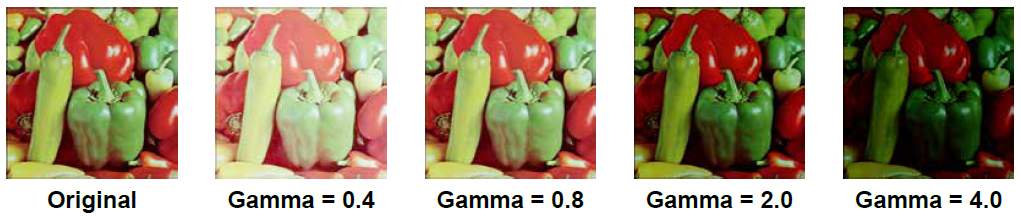
\includegraphics[width=1\linewidth]{FileAusiliari/Screenshots/Figure8-1.png}
    \caption{影像伽瑪校正演算法:當伽瑪值小於 1 時,影像會變得較亮;而當伽瑪值大於 1 時,影像會變得較暗。}
    \label{fig:gamma}
\end{figure}

\begin{figure}
    \centering
    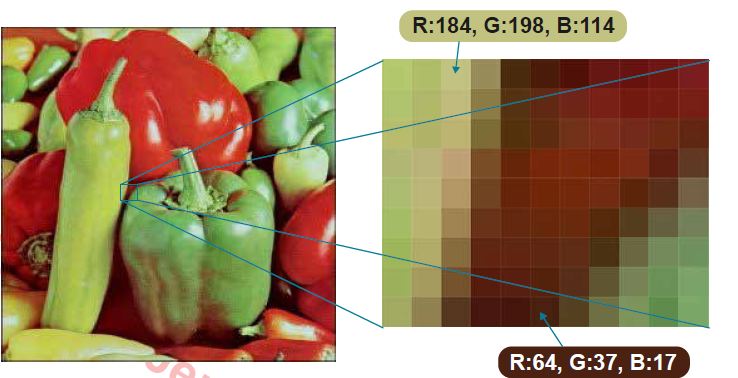
\includegraphics[width=0.9\linewidth]{FileAusiliari/Screenshots/Figure8-2.png}
    \caption{電腦化影像以像素的方式組成。彩色影像通常需要使用 RGB 亮度值來表示最終的像素顏色。}
    \label{fig:RGB}
\end{figure}

影像伽瑪校正是一種常見的影像處理演算法,用於調整影像的亮度而不改變其內容。如 \figref{fig:gamma} 所示,當應用的伽瑪值小於 1 時,影像會變得更亮;而當伽瑪值大於 1 時,影像會變暗。

儲存在電腦中的影像通常以像素的方式組成(見 \figref{fig:RGB})。像素是影像中的方形區域,每個像素用單一顏色渲染。例如,\figref{fig:gamma} 和  \figref{fig:RGB} 中的影像總共有 267(寬)× 267(高)個像素。如果影像是彩色的,則每個像素需要三個值分別表示紅色、綠色和藍色(RGB),這些值用於表示亮度。亮度通常以 8 個二進制整數(0–255)編碼,其中 0 表示最暗,255 表示最亮。另一種常見的方法是使用介於 0 和 1 之間的浮點數來表示亮度。所有像素的紅色亮度值組成「紅色頻道(channel)」,而彩色影像通常包含三個頻道(RGB)。

\begin{equation}
    V_{\text{out}} = V_{\text{in}}^{\gamma} \tag{8.1}
    \label{eq:gamma}
\end{equation}

影像伽瑪校正是一種逐位運算,對所有像素及其頻道應用簡單的浮點運算。如 \ref{eq:gamma} 所示,伽瑪值被用作亮度值的指數運算。伽瑪值大於 1 時,亮度值會降低。根據該公式,輸出的數值數量與輸入的數值數量一致,且每個輸出值的計算與相鄰值的計算相互獨立。影像伽瑪校正演算法是一種「高度平行化」的運算,因此非常適合於 GPU 實作。在此,我們提供了一個簡單的實作範例於程式 \lstref{lst:gamma} 中。

\begin{lstlisting}[language=C, caption={影像伽瑪校正應用作為一種「高度平行化」的演算法。每個執行緒(thread)負責處理影像像素陣列中的一個數值。Grid size 則反映了像素數量。}, captionpos=t, label={lst:gamma}]
#include <hip∕hip_runtime.h>
__global__ void image_gamma(uint8_t *d_image, float gamma, int num_values
 ) {
    int idx = threadIdx.x + blockIdx.x * blockDim.x;
    if (idx < num_values) {
        d_image[idx] = pow(d_image[idx] ∕ 255.0, gamma) * 255.0;
 }
}
int main() {
    int width, height, channels, num_values;
    uint8_t *data;

    ∕∕ 從檔案載入圖片

    int blockSize = 256;
    int gridSize = (num_values + blockSize - 1) ∕ blockSize;

    float gamma = 4.0;
    image_gamma<<<gridSize, blockSize>>>(
        d_image, gamma, num_values);

    hipMemcpy(data, d_image, num_values * sizeof(uint8_t),
        hipMemcpyDeviceToHost);

    ∕∕ 將圖片儲存到輸出檔案

    hipFree(d_image);
    return 0;
}
\end{lstlisting}

為了解決這個 GPU 程式設計問題,程式設計師必須首先考慮如何將執行緒對應到輸入和輸出元素。對於「高度平行化」的演算法,這樣的對應是直接且簡單的,因為每個執行緒負責輸出頻道的一部分(即一個像素)。因此,執行緒的總數將等於高度 × 寬度 × 頻道數 = \term{num\_values}。為了計算 grid size,我們將 \term{num\_values} 除以 block size。如果 block size 並非 \term{num\_values} 的倍數,我們可以將結果向上取整為下一個整數,如 \lstref{lst:gamma} 第 17 行所示。

Block size 可以介於 1 到 1,024 之間,具體取決於裝置的限制。需要注意的是,選擇合適的 block size 可以提升整體效能。根據 \figref{fig:BlockSize},當 block size 為 64 的倍數時,效能表現最佳,這是因為 AMD GPU 將 64 個執行緒組織為一個 wavefront,這是最小的資源分配單元。否則,CU 將被迫為每個 block 分配更多資源,導致效能下降。選擇 block size 為 64 的倍數,對於使用 AMD GPU 的「高度平行化」應用來說,可能是最佳的優化選擇。

\begin{figure}
    \centering
    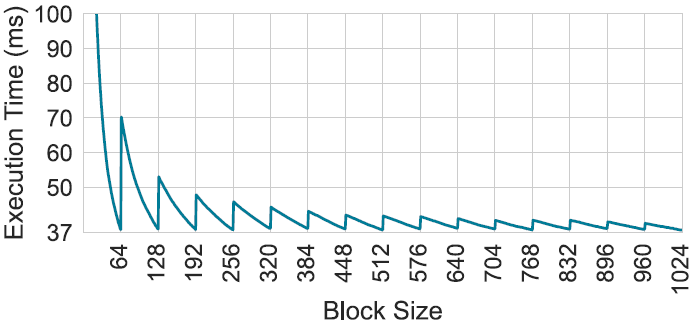
\includegraphics[width=0.9\linewidth]{FileAusiliari/Screenshots/Figure8-3.png}
    \caption{Block size 對程式效能的影響:影像伽瑪校正的執行時間基於 16,384 × 16,384 RGB 影像在 MI100 GPU 上的測試結果。}
    \label{fig:BlockSize}
\end{figure}

\section{Fixed-Sized Kernels—影像伽瑪校正} \label{sec:fixed_sized_kernels} 
在目前展示的大多數範例中,每個執行緒計算一個輸出元素。然而,仔細觀察可以發現,這樣的方式開銷較高,因為每個輸出元素都需要一個執行緒被分派到 CU,以計算全域 ID 並檢查邊界條件。為了降低這些開銷,我們將更多任務分配給每個執行緒,從而攤平在 GPU 上啟動執行緒的成本。

與其改變 grid size 來隨著輸入和輸出影像的大小成長,我們可以在 kernel 中固定工作群組的數量,並根據影像大小改變每個執行緒的工作量。在此,我們使用 Fixed-Sized kernels 重新實作影像伽瑪校正範例(見 \lstref{lst:FixedSize})。

這個新的實作方式與先前的版本相似,但有兩個小改動。首先,我們將 kernel 中的邊界檢查 IF 語句移到一個 FOR 迴圈中。這使得每個執行緒可以處理多個數值,並在每次迴圈中按執行緒總數遞增索引。例如,若有 640 個執行緒,0號執行緒將處理索引為 0、640、1,280 等的數值,而1號執行緒將處理索引為 1、641、1,281 等的數值。通過這樣的改變,我們可以根據問題大小靈活設置執行緒數量。

\begin{lstlisting}[language=C, caption={使用Fixed-Sized kernels 的影像伽瑪校正 GPU 實作: kernel 以預定義的大小啟動,每個執行緒負責處理影像中的多個像素。}, captionpos=t, label={lst:FixedSize}]
#include <hip∕hip_runtime.h>

__global__ void image_gamma(uint8_t *d_image, float gamma, int 
 num_values
 ) {
    int global_size = blockDim.x * gridDim.x;
    int idx = threadIdx.x + blockIdx.x * blockDim.x;
    for (; idx < num_values; idx += global_size) {
        float value = d_image[idx] ∕ 255.0f;
        value = pow(value, gamma);
        d_image[idx] = (uint8_t)(value * 255.0f);
    }
}

int main(int argc, char *argv[]) {
    int width, height, channels;
    uint8_t *data;

    ∕∕ 從檔案載入圖片

    int blockSize = 256;
    int gridSize = [Grid Size];

    float gamma = 4.0;
    image_gamma<<<gridSize, blockSize>>>(d_image, gamma, num_values);

    hipMemcpy(data, d_image, num_values * sizeof(uint8_t),
        hipMemcpyDeviceToHost);

    ∕∕ 將圖片儲存到磁碟

    return 0;
}
\end{lstlisting}

接下來,我們需要確定要使用的最佳 grid size。我們通過測量不同大小的 kernel 執行時間實驗來完成這項工作。結果如 \figref{fig:GridSize} 所示,我們觀察到四個主要趨勢。
首先,隨著工作群組數量的增加,效能會提高,因為當 work group 數量較少時,只有一部分 CU 被使用。其次,當 work group 數量達到 1,200(即 4,800 個 wavefront)時,效能達到飽和。這是 MI100 GPU 能夠平行處理的最大數量(120 個 CU × 40 個 wavefront = 4,800)。第三,使用 Fixed-Sized kernels 的最快執行時間為 15 毫秒。與這裡顯示的執行時間(至少 37 毫秒)相比,Fixed-Sized kernels 的實作將效能提升了 2.5 倍。這是因為 Fixed-Sized kernels 能減少 wavefront 調度的開銷。
最後,在 \figref{fig:GridSize} 中,執行時間呈現明顯的鋸齒模式。當工作群組數量達到 120 個 CU 的倍數後,執行時間會突然增加。當工作群組數量為 120 時,每個 CU 同時執行一個工作群組,因此可能會同時完成。少量的額外工作群組可能無法完全與前 120 個工作群組同時執行,並且會顯著增加 kernel 的執行時間。這是因為最後一組剩餘的工作群組可能無法充分利用 GPU,但仍需完成與第一組工作群組相同的任務量。這種效應被稱為「tail effect」,在 grid size 較小時尤為明顯,因此應盡可能避免。
總結來說,我們的實驗表明,Fixed-Sized kernels 可用於優化高度平行化的實作。最佳的工作群組大小應該是能填滿 GPU 所有 CU 的最小數量,並且始終是 CU 數量的倍數。

\begin{figure}[h]
    \centering
    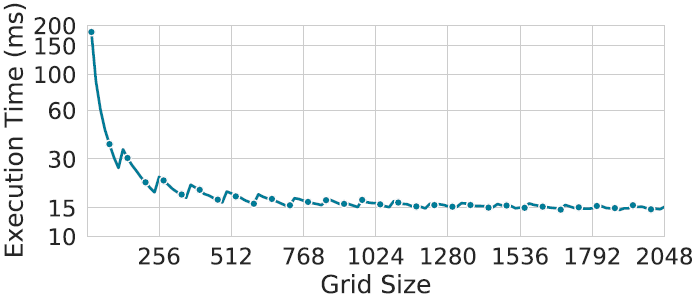
\includegraphics[width=0.9\linewidth]{FileAusiliari/Screenshots/Figure8-4.png}
    \caption{Grid size 對影像伽瑪校正程式效能的影響:執行時間基於在 MI100 GPU 上處理一張 16,384 × 16,384 RGB 影像的測量結果。}
    \label{fig:GridSize}
\end{figure}

\section{Reduce—陣列總和}
然而,並非所有 GPU 應用都屬於「高度平行化」的類型。舉個簡單的例子,如果我們需要計算一個陣列中的數值總和,就無法簡單地讓每個執行緒處理一個元素。在典型的 CPU 中,總和運算使用累加方式將元素逐一加入列表中,而這種演算法高度序列化,不適合在 GPU 上執行。因此,我們必須找到一種平行化的解決方案。

Reduction 操作可以通過計算陣列的總和來解決此類問題。其核心思想是最大化可用的平行化程度,同時仔細考慮裝置的使用效率。

化簡操作如 \figref{fig:reduce} 所示。我們將程式分為多個回合。在第一回合中,每個執行緒對相鄰的元素進行加總,將剩餘的元素數量減半。在第二回合中,執行緒數量再次減半。如此循環,直到最終只剩下一個總和。

\begin{figure}[h]
    \centering
    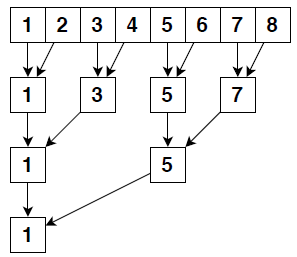
\includegraphics[width=0.4\linewidth]{FileAusiliari/Screenshots/Figure8-5.png}
    \caption{Reduction 程式設計。}
    \label{fig:reduce}
\end{figure}

在化簡模式中,一個實際的問題是執行緒之間必須互相傳遞資料。例如,在  \figref{fig:reduce} 中,第二回合中由3號執行緒計算的結果必須在第三回合中由1號執行緒讀取。如果將數據存回主記憶體(由 thread 3 存入),然後再由1號執行緒載入,將導致極高的開銷。理想情況下,我們希望將數據保存在 CU 中,以減少數據傳輸距離。

為了實現執行緒之間的通訊,最簡單的解決方案是使用 LDS 記憶體。LDS 是位於 CU 中的一部分可尋址記憶體,其結構類似於 L1 快取(cache),因此具有極低的延遲和高頻寬。LDS 記憶體中的數據可以在同一個 block 裡面的執行緒之間共享,因此可以加速化簡操作。

接下來,我們使用 \term{sum} kernel(見 \lstref{lst:sum})來展示如何利用 LDS 記憶體進行程式設計。

\begin{lstlisting}[language=C, caption={用 HIP 實作的程式,用於計算陣列中數字的總和。}, captionpos=t, label={lst:sum}]
#include <hip∕hip_runtime.h>

#include <iostream>
#include <vector>

const static int BLOCKSIZE = 256;

__global__ void reduction_sum(const float* input, float* output, 
 int size
 ) {
    int grid_size = blockDim.x * gridDim.x;

    ∕∕ 平行求和階段
    int idx = blockIdx.x * blockDim.x + threadIdx.x;
    float sum = 0;
    for (int i = idx; i < size; i += grid_size) {
        sum += input[i];
    }

    ∕∕ 將局部總和存入共享記憶體
    __shared__ float local_sum[BLOCKSIZE];
    local_sum[threadIdx.x] = sum;
    __syncthreads();

    ∕∕ Reduction 階段
    for (int s = BLOCKSIZE ∕ 2; s > 0; s ∕= 2) {
        if (threadIdx.x < s) {
            local_sum[threadIdx.x] += local_sum[threadIdx.x + s];
        }
    __syncthreads();
    }

    if (threadIdx.x == 0) {
        output[blockIdx.x] = local_sum[0];
    }
}

int main() {
    const static int N = 10485760;
    const static int num_blocks = 1200;

    std::vector<float> a(N);
    std::vector<float> b(num_blocks);

    ∕∕ 隨機化 a

    ∕∕ 分配裝置記憶體
    float* d_a;
    float* d_b;
    hipMalloc(&d_a, N * sizeof(float));
    hipMalloc(&d_b, num_blocks * sizeof(float));

    ∕∕ 將 a 複製到裝置記憶體
    hipMemcpy(d_a, a.data(), N * sizeof(float), hipMemcpyHostToDevice);

    ∕∕ 計算 a 的總和
    reduction_sum<<<num_blocks, BLOCKSIZE>>>(d_a, d_b, N);

    ∕∕ 將結果複製回主機記憶體
    hipMemcpy(b.data(), d_b, num_blocks * sizeof(float),
        hipMemcpyDeviceToHost);

    ∕∕ 完成總和計算
    hipDeviceSynchronize();
    float sum = 0;
    for (int i = 0; i < num_blocks; ++i) {
        sum += b[i];
    }

    ∕∕ 驗證結果
    double expected_sum = 0;
    for (int i = 0; i < N; ++i) {
        expected_sum += a[i];
    }
    if (abs(sum - expected_sum) > 1e-5 * expected_sum) {
        printf("Error: sum = %f, expected_sum = %f\n", sum, expected_sum);
    }
}
\end{lstlisting}

在此範例中,我們使用 Fixed-Sized kernels 實作 \term{sum} kernel。我們將 block size 設為 256,並啟動 1,200 個 block(如 \secref{sec:fixed_sized_kernels} 建議)。需要注意的是,陣列長度的變化不影響 block 的數量。

\term{Sum} kernel 分為兩個階段:平行加總和 reduce。在平行加總階段,每個執行緒會對列表中特定的元素進行加總。例如,第一個 kernel 會計算索引為 0、307,200、614,400 等的元素總和,因為根據 \lstref{lst:sum} 的程式碼,kernel 中有 256 × 1,200 = 307,200 個執行緒。完成平行加總後,我們將元素數量減少到 307,200。

接下來,我們使用 reduction algorithm 對剩餘的元素進行加總。Reduce 階段需要使用 LDS 記憶體,以實現 block 裡面執行緒之間的通訊。在第 19 行,我們首先使用 \bold{\_\_shared\_\_} 前綴在共享記憶體中分配一個暫存區(buffer),並且也為每個 block 分配共享記憶體暫存區。在此範例中,因為每個 block 有 256 個執行緒,每個執行緒使用 4-B 的單精度數據,因此每個 block 需要 256 × 4 = 1,024B 的 LDS 記憶體。隨後,block 裡面的執行緒會訪問該 block 擁有的暫存區中的數據。

讀寫 LDS 記憶體與讀寫全域記憶體的方式相同,如第 20 行所示。在這裡,我們將平行加總階段計算的總和存儲到共享記憶體中。

將數據寫入 LDS 記憶體後,我們必須調用 \term{\_\_syncthreads} 函數,這也被稱為「barrier」。Barrier 的作用是確保 block 裡面所有執行緒都完成執行特定的程式碼行後,才允許任何執行緒進行後續操作。如果沒有這個函數,block 裡面的不同 wavefront 可能會失去同步。如果某些執行緒仍在第 20 行執行,而其他執行緒已開始使用第 26 行的數據,結果可能會變得不一致。因此,LDS 記憶體操作通常需要與 barrier 結合使用,以確保正確的同步。

一個常見 barrier 使用的錯誤是將 barrier 放在條件語句內。因為 CU 會等待所有 wavefront 到達 barrier,但不會針對特定 wavefront 進行等待。根據 \lstref{lst:barrier} 的程式碼,其中一個 wavefront 執行第一個 IF 語句,另一個 wavefront 執行第二個 IF 語句。結果是第一個 wavefront 停在第 4 行,第二個 wavefront 停在第 9 行。然而,這並非我們期望的行為,因為同步應該在同一行程式碼上執行。為了避免這種情況,最簡單的解決方案是不將 barrier 放在條件語句內。

\begin{lstlisting}[language=C, caption={Barrier 不匹配的範例。}, captionpos=t, label={lst:barrier}]
__global__ void kernel() {
 if (global_id < 64) {
 ∕∕ 執行某些操作
 __syncthreads();
 }

 if (64 <= global_id && global_id < 128) {
 ∕∕ 執行某些操作
 __syncthreads();
 }
}
\end{lstlisting}

接下來,在第 23–29 行,我們執行化簡操作,直到將所有 256 個元素加總為一個結果。最後,我們使用每個 block 中的單一執行緒,將共享記憶體中的數據寫回全域記憶體。接著,陣列中的 307,200 個數字被加總為 1,200 個部分和。由於 block 間通訊的實現較為困難,我們依賴 CPU 來加總最後的 1,200 個數字,如 \lstref{lst:sum} 的第 62–64 行所示。

\section{Tiling 與 Reuse – 矩陣乘法}
矩陣乘法是 GPU 中最重要的工作負載之一,因為它支持許多計算問題。隨著深度神經網路(DNNs)的日益流行,矩陣乘法已變得至關重要,並且出現在神經網路中最計算密集的層中,例如全連接層(fully connected)和卷積層(convolutional)。在許多情況下,我們希望將問題轉化為使用矩陣乘法來解決,因為 GPU 已經針對矩陣乘法進行了高效優化。相比於原問題的迭代實現,矩陣乘法通常具有更高的效能~\cite{Parallel-multi-channel}。

\begin{figure}[h]
    \centering
    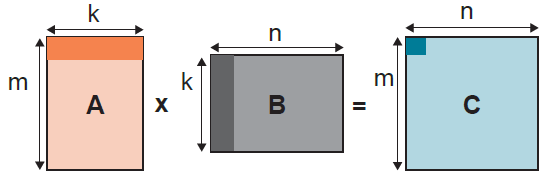
\includegraphics[width=0.7\linewidth]{FileAusiliari/Screenshots/Figure8-6.png}
    \caption{矩陣乘法運算。}
    \label{fig:MatrixMultiplication}
\end{figure}

如 \figref{fig:MatrixMultiplication} 所示,矩陣乘法運算涉及三個矩陣:A、B 和 C。矩陣 A 和 B 是輸入矩陣,而矩陣 C 是輸出矩陣。我們定義矩陣 A 有 \term{m} 行和 \term{k} 列,矩陣 B 有 \term{k} 行和 \term{n} 列。矩陣乘法要求 A 的列數等於 B 的行數。輸出矩陣 C 將繼承 \term{m} 行和 \term{n} 列。矩陣 C 中的每個元素是 A 的對應行和 B 的對應列中 \term{k} 個元素相乘後的總和,其公式如下所示:

\[
c_{ij} = a_{i1}b_{1j} + a_{i2}b_{2j} + \dots + a_{ik}b_{kj} = \sum_{l=1}^{k} a_{il}b_{lj}
\]
\[
\text{for } i = 1, \dots, n \text{ and } j = 1, \dots, m.
\]

一個迭代的 CPU 實作會使用三層巢狀迴圈來遍歷 \term{m}、\term{n} 和 \term{k}。每次迭代都執行一次乘法和累加運算。因此,理論上總共需要進行 \term{2mnk} 次運算。

相比之下,GPU 的實作是「高度平行化」的。GPU kernel 通過計算輸出矩陣中的每個元素來平行化 \term{m} 和 \term{n} 迴圈。因此,我們需要總共 \term{m×n} 個執行緒,每個執行緒執行一個包含 \term{k} 次迭代的迴圈。

儘管這種簡單的實作能夠產生正確的結果,但效能並不理想。對 kernel 執行進行分析顯示,GPU 從其 DRAM 中讀取的次數遠多於輸入矩陣的總大小。為了進一步探討這個問題,我們需要檢查執行緒是如何讀取輸入矩陣的。

\begin{lstlisting}[language=C, caption={簡單的 HIP kernel 用於矩陣乘法。}, captionpos=t, label={lst:naive}]
__global__ void matrix_multiply(float* a, float* b, float* out, size_t m, size_t n, size_t k) {
    int gidx = blockDim.x * blockIdx.x + threadIdx.x;
    int gidy = blockDim.y * blockIdx.y + threadIdx.y;

    if (gidx >= n && gidy >= m) {
        return;
    }

    float sum = 0;
    for (int i = 0; i < k; i++) {
        sum+= a[gidy * k + i] * b[i * n + gidx];
    }

    out[gidy * n + gid_x] = sum;
}
\end{lstlisting}

如 \figref{fig:memory} 所示,kernel 中的每個執行緒會讀取矩陣 A 的一整行和矩陣 B 的一整列。同一數據項可能會被來自不同 wavefront 的多個執行緒訪問。在我們的簡單實作中,所有的記憶體讀取操作都由主記憶體系統處理。儘管有多次對同一位置的重複記憶體引用,但這些記憶體訪問本應由快取處理。然而,由於快取空間有限且涉及的執行緒數量龐大,這對快取造成了巨大的記憶體壓力。隨著矩陣尺寸的增加,快取將無法容納這些數據,導致記憶體讀取操作被推送到主記憶體中,從而引起巨大的延遲。

理想情況下,GPU 程式設計者希望能對快取有更多的控制。當數據被加載到快取中時,應該在釋放之前盡可能多地被執行緒重複使用。在 CPU 程式設計中,快取對程式設計者是無法控制的。但與之不同的是,GPU 提供了 LDS 記憶體,它實際上是一個可編程的 L1 快取。

為了使用 LDS 改善矩陣乘法的效能,我們應用了一種常見的 GPU 程式設計技術,稱為「tiling」。Tiling 方法利用工作群組中的所有執行緒共同處理部分數據,然後再移動到問題的下一部分。如 \figref{fig:tiling} 所示,第一個工作群組將矩陣 A 和 B 藍色區塊中的數據加載到 LDS 中,接著對加載的區塊進行矩陣乘法運算。然後,wavefront 移動到橙色區塊,繼續累加乘法結果。

\begin{figure}[h]
    \centering
    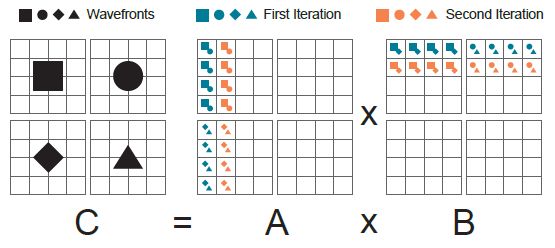
\includegraphics[width=0.7\linewidth]{FileAusiliari/Screenshots/Figure8-7.png}
    \caption{矩陣乘法 GPU kernel 中簡單實作的記憶體存取模式,該模式顯示所有數據項會被多次載入。}
    \label{fig:memory}
\end{figure}

\begin{figure}[h]
    \centering
    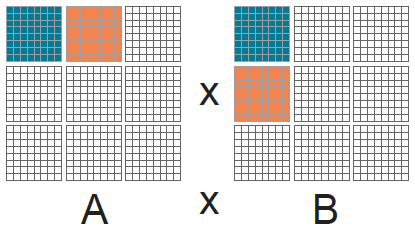
\includegraphics[width=0.6\linewidth]{FileAusiliari/Screenshots/Figure8-8.png}
    \caption{使用 tiling 技術加速矩陣乘法 GPU kernel。}
    \label{fig:tiling}
\end{figure}

\begin{lstlisting}[language=C, caption={基於 tiling 的 HIP kernel 用於矩陣乘法。}, captionpos=t, label={lst:tiling}]
__global__ void matrix_multiply_tile(float *A, float *B, float *Out,
 int m, int n, int k) {
    __shared__ float subTileA[TileSize][TileSize];
    __shared__ float subTileB[TileSize][TileSize];

    int bx = blockIdx.x;
    int by = blockIdx.y;
    int tx = threadIdx.x;
    int ty = threadIdx.y;

    int row = by * TileSize + ty;
    int col = bx * TileSize + tx;

    float sum = 0;
    for (int i = 0; i < ((k - 1) ∕ TileSize + 1); i++) {
        int a_index = row * k + i * TileSize + tx;
        int b_index = (i * TileSize + ty) * n + col;

        if (i * TileSize + tx < k && row < m) {
            subTileA[ty][tx] = A[a_index];
        } else {
            subTileA[ty][tx] = 0.0;
        }

        if (i * TileSize + ty < k && col < n) {
            subTileB[ty][tx] = B[b_index];
        } else {
            subTileB[ty][tx] = 0.0;
        }

        __syncthreads();

        for (int j = 0; j < TileSize; j++) {
            if (j + TileSize * i < k) {
                sum += subTileA[ty][j] * subTileB[j][tx];
            }
        }

    __syncthreads();
    }

    if (row < m && col < n) {
        Out[row * n + col] = sum;
    }
}
\end{lstlisting}

基於 tiling 的 kernel 實作如 \lstref{lst:tiling} 所示。該 kernel 的接口與簡單實作完全相同。唯一的特別要求是必須定義 macro \term{TileSize},以確定在每個維度中要分組為單一 block 的元素數量。工作群組大小必須與 block 大小相匹配,以確保輸出的正確性。

Kernel 的實作也必須修改為使用兩個 FOR 迴圈,而不是僅使用一個。外層迴圈負責處理跨 block 的記憶體,而內層迴圈則進行乘法和累加操作。在迴圈開始之前,我們為矩陣 A 和 B 的 block 分別分配了兩個 buffer:一個在 \lstref{lst:tiling} 的第 3 行,另一個在第 4 行。在外層迴圈的每次迭代中,我們將數據從主記憶體加載到 LDS,如第 20–26 行所示。這裡,實作的複雜性主要來自於索引計算和邊界檢查。接下來,我們使用內層迴圈,類似於簡單實作中的方式,來執行乘法和累加操作。需要注意的是,在內層迴圈的前後必須設置 barrier,分別確保所有數據已加載和已被使用。最後,在第 43 行,我們將最終結果存儲到輸出矩陣中。

Tiling 是一種有效減少 DRAM 存取並提升效能的方法。在我們的範例中,當在 MI50 GPU 上執行矩陣乘法,且 \term{m}=\term{n}=\term{k}=8,192 時,簡單實作需要 1.60 秒,而使用 tiling 後,kernel 僅需 0.76 秒,實現了 2.1 倍的效能提升。

\section{Tiling 與合併 : 矩陣轉置}
矩陣轉置是一個基本的線性代數計算,也是許多任務的基本操作。矩陣轉置並不涉及複雜的計算,而是僅僅涉及記憶體的移動。由於 GPU 通常比 CPU 擁有顯著更高的記憶體頻寬,因此在執行矩陣轉置操作時,GPU 具有獨特的優勢。
與之前的範例類似,矩陣轉置是一種高度平行的實現方式(參見 \lstref{lst:transpose}),其中每個執行緒負責移動一個矩陣元素。

\begin{lstlisting}[language=C, caption={簡單矩陣轉置的 kernel 範例。}, captionpos=t, label={lst:transpose}]
__global__ void matrix_transpose_simple(float *in, float *out,
int width, int height)
int x_index = blockIdx.x * tile_dim + threadIdx.x;
int y_index = blockIdx.y * tile_dim + threadIdx.y;

int in_index = y_index * width + x_index;
int out_index = x_index * height + y_index;

out[out_index] = in[in_index];
\end{lstlisting}

我們對 MI50 GPU 上執行的 16,384 × 16,384 矩陣轉置進行 kernel 效能分析。接著,利用分析工具的指標 \term{TCC\_EA\_WRREQ\_sum} 和 \term{TCC\_EA\_RDREQ\_sum},我們可以分別檢查對 DRAM 的讀取和寫入總數。理論上,矩陣轉置的讀取與寫入次數應該大致相等,因為從輸入矩陣中讀取的所有資料都會被寫回。然而,分析結果顯示 kernel 的寫入次數遠多於讀取次數(1,551,894 次寫入對比 524,288 次讀取)。

\begin{figure}[h]
    \centering
    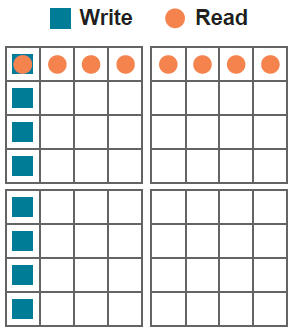
\includegraphics[width=0.4\linewidth]{FileAusiliari/Screenshots/Figure8-9.png}
    \caption{簡單記憶體轉置 kernel 實現的記憶體訪問模式。}
    \label{fig:transpose}
\end{figure}

為了了解為什麼 kernel 會寫入更多數據,我們需要深入檢查記憶體訪問模式。矩陣轉置 kernel 不太可能像矩陣乘法 kernel 一樣,造成重複訪問記憶體的問題,因為每個元素只會被訪問一次。因此,問題應該出現在相關讀取和寫入操作的地址模式上。

在 \figref{fig:transpose} 中,我們展示了 kernel 執行緒訪問的數據。在我們的實作中,相鄰的執行緒會水平地讀取數據,並垂直地寫入數據。由於我們使用的是row-major 矩陣,相鄰的執行緒會從相鄰的地址讀取數據,但寫入數據時使用了較大的地址跨度(即兩個連續地址之間的差異)。正如我們在 \secref{sec:memory_coalescing}  中解釋的,如果地址落在同一個 cache line 中,GPU 可以將記憶體訪問合併以減少總訪問次數。在矩陣轉置 kernel 中,讀取操作是可以合併的,但寫入操作無法合併。因此,我們自然會觀察到 DRAM 的寫入次數多於讀取次數。

我們可以使用 LDS 將無法合併的記憶體訪問轉換為可合併的訪問。如 \figref{fig:lds} 所示,我們將矩陣轉置過程分為兩個步驟。首先,我們將數據從輸入矩陣移動到 LDS 記憶體。在此過程中,我們水平讀取數據,確保記憶體訪問是合併的。當 LDS 暫存區填滿後,我們再將數據從 LDS 移動到主記憶體。在這一步中,我們垂直讀取數據並水平寫入數據。由於 LDS 記憶體的頻寬明顯高於全域記憶體,因此無論是水平還是垂直讀取數據,都不會影響整體效能。然而,我們水平寫入數據,確保寫入主記憶體的操作也是合併的。藉此,我們將 LDS 作為輸入矩陣與輸出矩陣之間的中介數據傳輸緩衝區,使讀取和寫入操作都能實現合併訪問。

\begin{figure}[h]
    \centering
    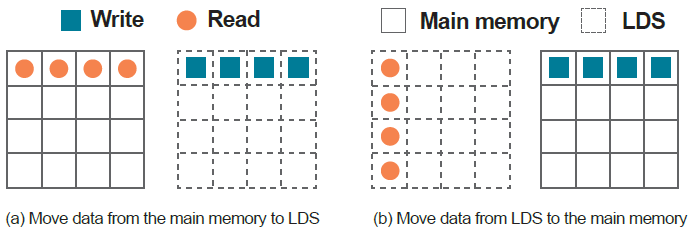
\includegraphics[width=0.8\linewidth]{FileAusiliari/Screenshots/Figure8-10.png}
    \caption{使用 LDS 避免非合併記憶體訪問。}
    \label{fig:lds}
\end{figure}

\begin{lstlisting}[language=C, caption={使用 LDS 的矩陣轉置 kernel 範例。}, captionpos=t, label={lst:transpose}]
__global__ void matrix_transpose_lds(float *in, float *out,
 int width, int height) {
 __shared__ float tile[tile_dim][tile_dim];

 int x_tile_index = blockIdx.x * tile_dim;
 int y_tile_index = blockIdx.y * tile_dim;

 int in_index = (y_tile_index + threadIdx.y) * width +
 (x_tile_index + threadIdx.x);
 int out_index = (x_tile_index + threadIdx.y) * height +
 (y_tile_index + threadIdx.x);

 tile[threadIdx.y][threadIdx.x] = in[in_index];

 __syncthreads();

 out[out_index] = tile[threadIdx.x][threadIdx.y];
}
\end{lstlisting}

\section{結語}
在本章中,我們使用多種應用範例來說明設計 GPU kernel 時的重要考量,以優化 GPU 程式的效能。我們從簡單的工作負載(例如影像伽馬校正)開始,討論如何透過固定每個執行緒工作負載和固定 kernel 大小的解決方案,來組織高度平行的 GPU 工作負載。這些範例充分展示了選擇最佳 block size 對 kernel 實現效能的影響。

其次,我們專注於優化 kernel 以更好地適應 GPU 記憶體系統的特性,特別是 LDS 記憶體。透過使用 LDS 記憶體,我們可以提升 ALU 的使用率(例如陣列總和)、減少記憶體訪問次數(例如矩陣乘法),以及實現記憶體合併(例如矩陣轉置操作)。